% Simple poster (portrait)
% Author: Sofia Jijon (https://sjijon.github.io)
% Last Update: Sept 9, 2021
% Latest Version: https://github.com/sjijon/TeX-templates/tree/main/Tikzposter%20posters/Simple%20poster

\documentclass[a0paper,portrait,margin=0pt, colspace=24pt,subcolspace=0pt,blockverticalspace=36pt,innermargin=50pt]{tikzposter}

\usepackage[latin9]{inputenc}
\usepackage[square,numbers]{natbib} 	% Bibliography manager
\usepackage{amsmath,amssymb}
\usepackage{lipsum} 
% Random Text
\usepackage[colalign]{aligncolsatbottom}  %To align columns at bottom (!! please run 2 times)

%..............................................................................................................................................................................................
% Display
\tikzposterlatexaffectionproofoff 			
\usetikzlibrary{shapes.geometric,arrows.meta,positioning}  %Tikz Libraries

% Fonts
\usepackage{helvet}					% Sans-Serif
\renewcommand{\familydefault}{\sfdefault}	%

% Colors
	\definecolor{MyOrange}{rgb}{0.8, 0.33, 0}
	\definecolor{MyBrown}{rgb}{0.28, 0.20, 0.20}
	\definecolor{MyGreen}{rgb}{0.33, 0.42, 0.18}

% Theme
\usetheme{Default}
\definecolorstyle{MyStyle2016}{
	\definecolor{ColorOne}{named}{MyBrown} 
	\definecolor{ColorTwo}{named}{MyOrange}
	\definecolor{ColorThree}{named}{MyGreen}
}{
    % Title Colors
    \colorlet{titlebgcolor}{ColorOne}
    \colorlet{titlefgcolor}{white}
    % Background Colors
    \colorlet{backgroundcolor}{ColorOne!15}
    \colorlet{framecolor}{ColorOne}
    % Block Colors
    \colorlet{blocktitlebgcolor}{white}
    \colorlet{blocktitlefgcolor}{ColorTwo}
    \colorlet{blockbodybgcolor}{white}
    \colorlet{blockbodyfgcolor}{black}
    % Innerblock Colors
    \colorlet{innerblocktitlebgcolor}{ColorOne!15}
    \colorlet{innerblocktitlefgcolor}{black}
    \colorlet{innerblockbodybgcolor}{ColorOne!15}
    \colorlet{innerblockbodyfgcolor}{black}
    % Note colors
    \colorlet{notebgcolor}{ColorTwo!20}
    \colorlet{notefgcolor}{ColorTwo}
    \colorlet{notefrcolor}{ColorTwo}
 }

% Color style
\usecolorstyle{MyStyle2016}
%..............................................................................................................................................................................................
\title{\parbox{\linewidth}{\centering Introduction to Conformal Prediction with Application on Imbalanced \\ Diabetes Classification}}


\author{Mabrouka Salmi\textsuperscript{1}} \institute{	\textsuperscript{1}Universidad de Cordoba, Cordoba, Spain. z12salsm@uco.es}

%..............................................................................................................................................................................................
\begin{document}
%
%
%	HEAD
%
%....................................................................................
%
%	Title
%
\maketitle[width=0.96\linewidth,titletoblockverticalspace=36pt,linewidth=0,roundedcorners=10]
%..............................................................................................................................................................................................
%
%	LEFT COLUMN
%
\begin{columns}
\column{0.33}
%....................................................................................
%
%	Block
%
\block[titleleft,roundedcorners=16]{Introduction}{
	\raggedright
Traditional machine learning methods provide single value predictions without indicating the confidence or reliability of these predictions \cite{toccaceli2022introduction}. Conformal prediction (CP) addresses this limitation by producing prediction sets or intervals that come with a measure of their accuracy and reliability, thereby guaranteeing a given error rate \cite{gammerman2007hedging}. CP methods rely on minimal assumptions, such as the test data being drawn from the same distribution as the training data and the exchangeability of the data points \cite{toccaceli2019combination}.

Non-conformity measures (NCMs) are used to assess how unusual a new example is compared to the training examples. Based on the NCM, the CP framework generates prediction sets by evaluating the randomness of hypothetical completions of test examples and including only those labels that meet a predefined significance level.

The validity of CPs is ensured by calculating p-values for hypothetical completions and forming prediction sets that reflect a chosen confidence level. CPs aim for a balance between validity (ensuring error rates do not exceed the significance level) and efficiency (keeping prediction sets as small as possible without missing correct labels).
}
%....................................................................................
%
%	Block
%
\block[titleleft,roundedcorners=16]{Background}{
	\raggedright
\textbf{Transductive and Inductive CP Algorithms}

	Inductive conformal prediction (ICP) splits the training data into training and calibration sets. After training a model, nonconformity scores are calculated for both sets. These scores are ordered, and the significance level $\alpha$ is chosen. The prediction intervals are constructed as $\hat{y} \pm \alpha_s$, where $\alpha_s$ is the $(1 - \alpha)$ percentile of the nonconformity scores. In classification, nonconformity scores, similar to p-values, indicate the probability of more extreme outcomes under the null hypothesis.

	Transductive conformal prediction (TCP) uses all available data without needing a separate calibration set, leveraging the entire dataset for efficient and precise interval predictions. Nonconformity measures, such as absolute error for regression tasks or Hinge loss for binary classification, are selected based on the problem:

	\[
	\text{Non-conformity score: } \alpha = |y - \hat{y}|\]

	\[
	\text{Non-conformity score: }  \alpha = 1 - P(y|x)\]

	The model is trained on the entire dataset, and nonconformity scores for hypothetical completions are calculated. P-values are computed to determine the statistical significance of these scores, guiding the inclusion of hypothetical completions in the prediction set based on the chosen significance level $\alpha$.

	\textbf{Label-Conditional Conformal Prediction}

	Label-conditional conformal prediction (Mondrian CP) constructs prediction intervals based on the conditional probability of labels given features. Nonconformity scores are computed conditioned on the predicted label:

	\[
	\alpha(\mathbf{x}, y) = \text{deviation between expected output}\\ \text{ and true label}
	\]

	P-values for test objects with hypothetical labels are calculated, considering only examples with the same label as the hypothetical label. This approach leads to more accurate and calibrated prediction sets, especially when the conditional distribution of labels varies significantly across instances.

}
%....................................................................................
%

%..............................................................................................................................................................................................
%
%	CENTER COLUMN
%
\column{0.34}
%....................................................................................
%
% 	Block
%
\block[titleleft,roundedcorners=16]{Methodology}{
	\raggedright
We want to experiment with CP for the classification learning task. We use the three common classical conformal prediction algorithms: the transductive or full conformal prediction, the inductive conformal prediction, and the label conditional conformal prediction.  We interestingly experimented with conformal prediction for imbalanced data, which is not well explored yet, particularly in medical diagnosis applications. First, we select an imbalanced medical data set to expose the inductive and transductive algorithms for imbalanced classification. Then, to better evaluate the conformal prediction on imbalanced data, a simple random forest classifier is used as a baseline performance to compare the results of the classification of patient cases.
}
\block[titleleft,roundedcorners=16]{Experimental work and Results}{
    \raggedright
\subsection{Used Dataset and Evaluation}
	The Pima Indian diabetes dataset, obtained from the UCI Repository, is a popular benchmark \cite{chang2023pima}. It presents classification challenges due to its moderate imbalance and small sample size. Data was split for CP algorithms as follows:
	\begin{itemize}
	    \item \textbf{Transductive CP}: 80-20 train-test split.
	    \item \textbf{Inductive CP}: 70-15-15 train-calibration-test split.
	\end{itemize}
	
	The Random Forest classifier, capable of handling continuous and discrete variables, was used. CP models were evaluated for validity and efficiency:
	\begin{itemize}
	    \item \textbf{Validity}: Ensured by CP framework.
	    \item \textbf{Efficiency}: Measured by the informativeness of predictions.
	    \item \textbf{Metrics}: Accuracy, mean error of classification, and number of single class predictions.
	\end{itemize}    
\subsection{Results}
	We applied three conformal prediction algorithms based on the Random Forest classifier: transductive CP, inductive CP, and label-conditional CP. The Random Forest classifier was trained on the train data and used to produce test set predictions. The table below displays the CP models and the efficiency and validity metrics scores of their predictions. All related code is available on this GitHub repository \cite{Bouka2023} to share further related investigations.
    \vspace{1cm}
	\begin{center}
	\centering
	\label{tab1}
	\begin{tabular}{|l|l|l|}
	\hline
	CP Model\textbackslash{}Metric & \textbf{Err Rate} & \textbf{Avg C/pred} \\ \hline
	\textbf{Inductive CP}          & 0.1034              & 1.30                                              \\ \hline
	\textbf{Transductive CP}       & 0.1168              & 1.3311                                            \\ \hline
	\textbf{Label-Conditional CP}  & 0.1168              & 1.3831                                            \\ \hline
	\end{tabular}
           \\
     Note: Avg C/pred: Average number of classes per prediction; Err Rate: Error Rate
    
	\end{center}
\vspace{1cm}
	To compare the performance of the CP and non-CP models, we refer to calculating the accuracy of the predictions of the test set. Figure \ref{fig1} plots the accuracies of each CP and random forest model. Accordingly, we see the higher performance achieved by the CP models.
 	\begin{center}
		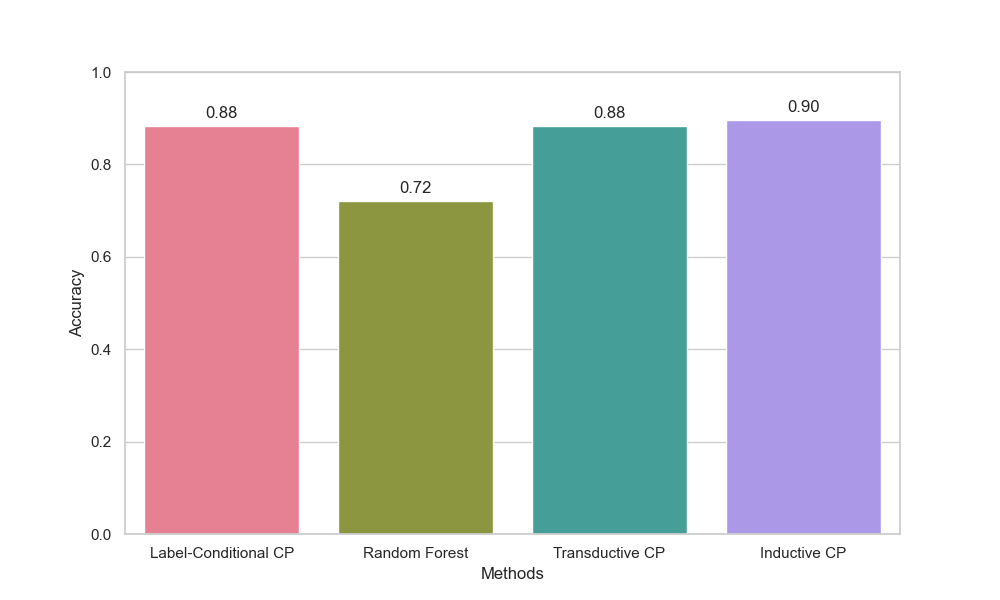
\includegraphics[width=0.9\linewidth, height=13cm]{Figure_1.png}
  \label{fig1}
	\end{center}
	
	


 }
%....................................................................................
%
%	Block
%

%..............................................................................................................................................................................................
%
% 	RIGHT COLUMN
%
\column{0.33}
%%....................................................................................
%
%	Block
%
\block[titleleft,roundedcorners=16]{Discussion}{
	\raggedright
The CP algorithms for the diabetes classification have surpassed the random forest classifier regarding prediction accuracy. However, the three employed CP algorithms present slight differences between them. The inductive CP has produced the most accurate diabetes classification results with the least error rate and the highest accuracy. Although the difference could be noticed concerning the error rate, the efficiency measure shows almost similar values referring to insignificant differences in CP model efficiency. Moreover, as seen in figure \ref{fig1}, the CP models not only showed good accuracy values and relatively low error rates, but the performance of the build CP models also exceeds that of the models proposed in the most recent experimental research with different ML algorithms for Indian diabetes classification \cite{chang2023pima}. The accuracy of the optimal classification model in that research is around 80\%. Then, the CP models trained for CP trials on class imbalance data within this work have largely improved the performance of Pima diabetes classification without reference to class imbalance data level methods. Such preliminary results are promising for further experimentation with imbalanced data and validating the CP performance in different dataset configurations.
	
	}
%....................................................................................
%
%	Block
%
\block[titleleft,roundedcorners=16]{Conclusions}{
	\raggedright
The evolving conformal prediction approach for soft computing helps provide informative predictions for future objects without relying on past object distribution or parametric methods. Such an agnostic model approach could be adapted to the problem and the data. Besides, its validity property is guaranteed regardless of the underlying machine learning algorithm or non-conformity measure. Recent research is focused on broadening the usage of such methods in different contexts and problems like image and time series data. Hence, even when data assumptions are violated, the CP could still be adapted to various scenarios. In our empirical work with Pima Indian diabetes, one of the challenging benchmark datasets, it is revealed that CP models considerably improved the classification results and significantly outperformed the state-of-the-art results. As was expected, the CP models based on random forest outperformed the non-CP random forest. Finally, these preliminary results should be completed with a thorough evaluation of the CP classifiers on various imbalanced datasets regarding data size and imbalance degree. 
 }

%\end{columns} 
%..............................................................................................................................................................................................
%
%	FOOT
%
%....................................................................................
%
%	References
%
\block[titleleft,roundedcorners=16]{}{
\small
\begin{minipage}{0.73\linewidth}
	\nocite{*}
	\bibliographystyle{unsrtnat}
	\bibliography{BibPoster}
 \end{minipage}}
 \end{columns} 
%....................................................................................
%

%....................................................................................
%
%	My info
%

\end{document}